\section*{1}

\begin{enumerate}[label=\Alph*]
    
\item Resuelva gráficamente el siguiente problema de optimización:
        \begin{equation*}
        \begin{aligned}
            \text{Minimizar }   & x_1^2 + x_2^2 \\
            \text{sujeto a }    & x_1 \geq 0,\; x_2 \geq 0, \\
                                & x_1 x_2 \geq 1 \\
                                & x_1 + x_2 \geq 4 \\
        \end{aligned}
        \end{equation*}

\item Resuelva, ahora, el problema de maximización con la misma función objetivo y el mismo conjunto factible del apartado anterior. 

\end{enumerate}

\noindent\rule{10cm}{0.4pt}

Usando \textit{Python} junto a \textit{matplotlib} creamos un gráfico con curvas de nivel sobre el conjunto factible,
para ello damos un valor de $+\infty$ a los puntos que no cumplan con las restricciones.

Como vemos en la figura \ref{ex0_min} el mínimo se encuentra en el punto $(2, 2)$.

\begin{figure}[h]
\centering
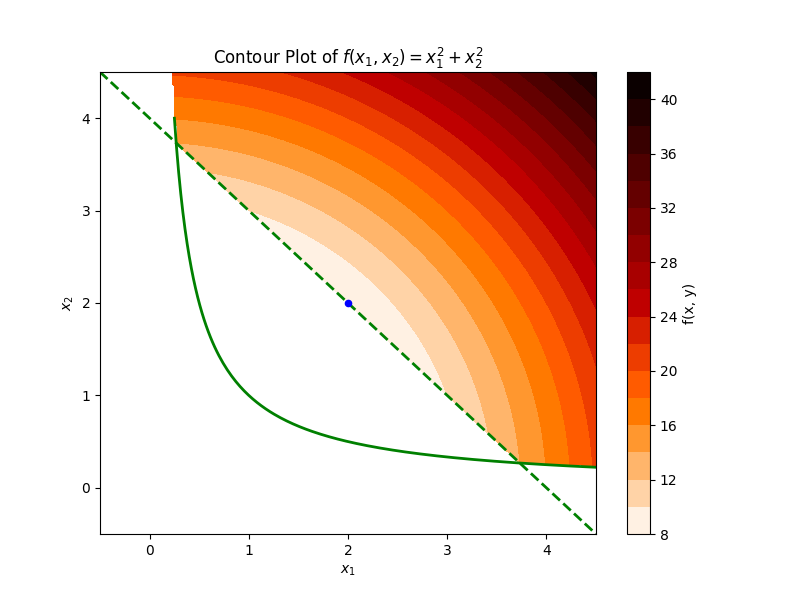
\includegraphics[scale=0.6]{ex0_min.png}
\caption{Solución gráfica para el problema de minimizar.}
\label{ex0_min}
\end{figure}

Para resolver el problema de maximización damos un valor de $-\infty$ a los puntos que no cumplan las restricciones.
Como se ve en la figura \ref{ex0_max} el funcional no esta acotado en el conjunto factible,
por tanto no tiene solución.

\begin{figure}[h]
\centering
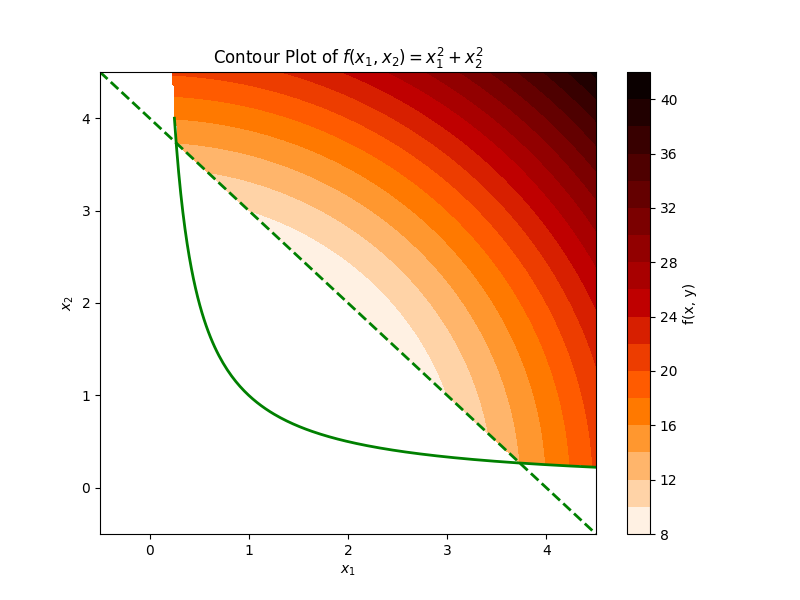
\includegraphics[scale=0.6]{ex0_max.png}
\caption{Solución gráfica para el problema de maximización.}
\label{ex0_max}
\end{figure}

